\documentclass[conference]{IEEEtran}

\usepackage[]{graphicx}    % We use this package in this document
\usepackage{amsmath}
\usepackage{mathtools}
\usepackage{subfiles}
\usepackage{amssymb}
\usepackage{hyperref}
\usepackage{algorithm}

\usepackage{tikz,tikz-3dplot}
\usepackage{pgfplots}
\usepackage{subcaption}
\usepackage{arevmath}     % For math symbols
\usepackage[noend]{algpseudocode}
\usepackage[margin=1.5in]{geometry}    % For margin alignment
\usepackage[english]{babel}
\usepackage[utf8]{inputenc}
\usepackage{tabularx,booktabs}
\usepackage{listings}

% \newcolumntype{C}{>{\centering\arraybackslash}X} % centered version of "X" type


\newcommand{\ignore}[1]{}  % {} empty inside = %% comment
\graphicspath{ {./pics/} }

% \ifCLASSINFOpdf
% \else
% \fi

\hyphenation{op-tical net-works semi-conduc-tor}


\begin{document}

\title{Heterogenous Autonomous Robotic Exploration (HARE)}

\author{Jackson~Parker, Allen~Spain, Caleb~Adams}

% The paper headers
% \markboth{IEEE JOURNAL XXXX, VOL. XX, NO. XX, MONTH 20XX}%
% {Shell \MakeLowercase{\textit{et al.}}: Bare Demo of IEEEtran.cls for IEEE Journals}

% \markboth{IEEE JOURNAL OF SELECTED TOPICS IN APPLIED EARTH OBSERVATIONS AND REMOTE SENSING, VOL. XX, NO. XX, MONTH 20XX}



% If you want to put a publisher's ID mark on the page you can do it like
% this:
%\IEEEpubid{0000--0000/00\$00.00~\copyright~2015 IEEE}
% Remember, if you use this you must call \IEEEpubidadjcol in the second
% column for its text to clear the IEEEpubid mark.



% use for special paper notices
%\IEEEspecialpapernotice{(Invited Paper)}




% make the title area
\maketitle
\thispagestyle{plain}
\pagestyle{plain}

% As a general rule, do not put math, special symbols or citations
% in the abstract or keywords.
\begin{abstract}
  The purpose of this research is to prove that subtask division can be accomplished based on knowledge of robot capabilities. To prove this, we are developing an exploration system in which robots with different hardware and capabilities will work together to accurately explore and map a complex region of space. Through the definition of individual attributes and the sharing of those attributes, each robot will search and map regions of space that it is capable of maneuvering. Instead of simple indexed mapping of the region where each cell on the map is represented by and index, each robot will mark the region that it has explored and can maneuver through this a specific identifier. The robots share sensed terrain using map node which defines the region in terms of terrain. This gives the state space provides the following information that can enable a robot to determine it's terrain, traversability (as determined by groups attributes). After the region has been sensed it is also marked as explored which is factored in when determining tree state. See table below for implemented terrain definitions, see table \ref{tabl:terrain} in appedix.
  Once a robot comes to an obstacle or region that it cannot maneuver around, it will evaluate which team members are capable of doing so and mark that space for the capable robots to explore. Due to time limitations on this project, instead of relying on complex perceptive capabilities to evaluate which robots could explore that region, the utilization of terrain identification which can be surveyed by the robot's sensors to determine if a region is traversable, this is designed statically in this experiment as a proof of concept. However, the proposed concept allows robots to compare their own attributes with those required to traverse a terrain in the sensed region. The robot attributes for the general case is shown in table \ref{tabl:attributes}.

  \begin{figure}[H]
    \centering
      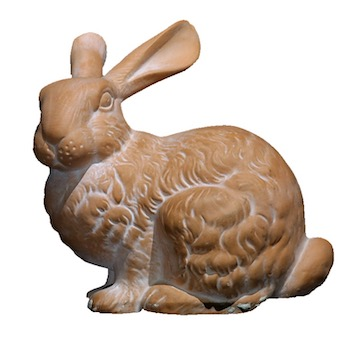
\includegraphics[width=0.2\textwidth]{hare-rabbit}
    \caption{The wild hare known for its swiftness, stamina and adaptability.}
    \label{fig:hare-rabbit}
  \end{figure}


\end{abstract}


% Note that keywords are not normally used for peerreview papers.
\begin{IEEEkeywords}
IEEE, IEEEtran, journal, \LaTeX, paper, template, multi-robot systems, exploration, autonomous mobile robots, heterogenous, breadth-first search,path planning, behavior trees
\end{IEEEkeywords}


\IEEEpeerreviewmaketitle

\begin{figure}[H]
  \centering
    \includegraphics[width=0.5\textwidth]{hare}
  \caption{High level block diagram for HARE}
  \label{fig:something3}
\end{figure}

%%%%%%%%%%%%%%%%%%%%%%%%%%%%%%%%%%%%%%
\section{Introduction}
%%%%%%%%%%%%%%%%%%%%%%%%%%%%%%%%%%%%%%
\subfile{tex/intro}

%%%%%%%%%%%%%%%%%%%%%%%%%%%%%%%%%%%%%%%%%%%
\section{Methodology}
%%%%%%%%%%%%%%%%%%%%%%%%%%%%%%%%%%%%%%%%%%%
\subfile{tex/methodology} %  <-- might be best to keep the example and remake some subfiles

%%%%%%%%%%%%%%%%%%%%%%%%%%%%%%%%%%%%%%%%%%%
\section{Results}
%%%%%%%%%%%%%%%%%%%%%%%%%%%%%%%%%%%%%%%%%%%
\subfile{tex/results} %  <-- might be best to keep the example and remake some subfiles

%%%%%%%%%%%%%%%%%%%%%%%%%%%%%%%%%%%%%%%%%%%
\section{Conclusion}
%%%%%%%%%%%%%%%%%%%%%%%%%%%%%%%%%%%%%%%%%%%
\subfile{tex/conclusion} %  <-- might be best to keep the example and remake some subfiles


% use section* for acknowledgment
\subfile{tex/appendix}
% \section*{Acknowledgment}

% \ifCLASSOPTIONcaptionsoff
%   \newpage
% \fi
%
% \bibliographystyle{IEEEtran}
% \bibliographystyle{/Users/allenspain/Documents/Development/hare doc/latex_MRS/sources}

\bibliographystyle{IEEEtran}
\bibliography{sources}
\newline
% \bibliography{sources}
% \bibliography{IEEEabrv,sources} % ftp://tug.ctan.org/pub/tex-archive/macros/latex/contrib/IEEEtran/bibtex/IEEEtran_bst_HOWTO.pdf


% insert where needed to balance the two columns on the last page with
% biographies
% \newpage

\begin{IEEEbiography}{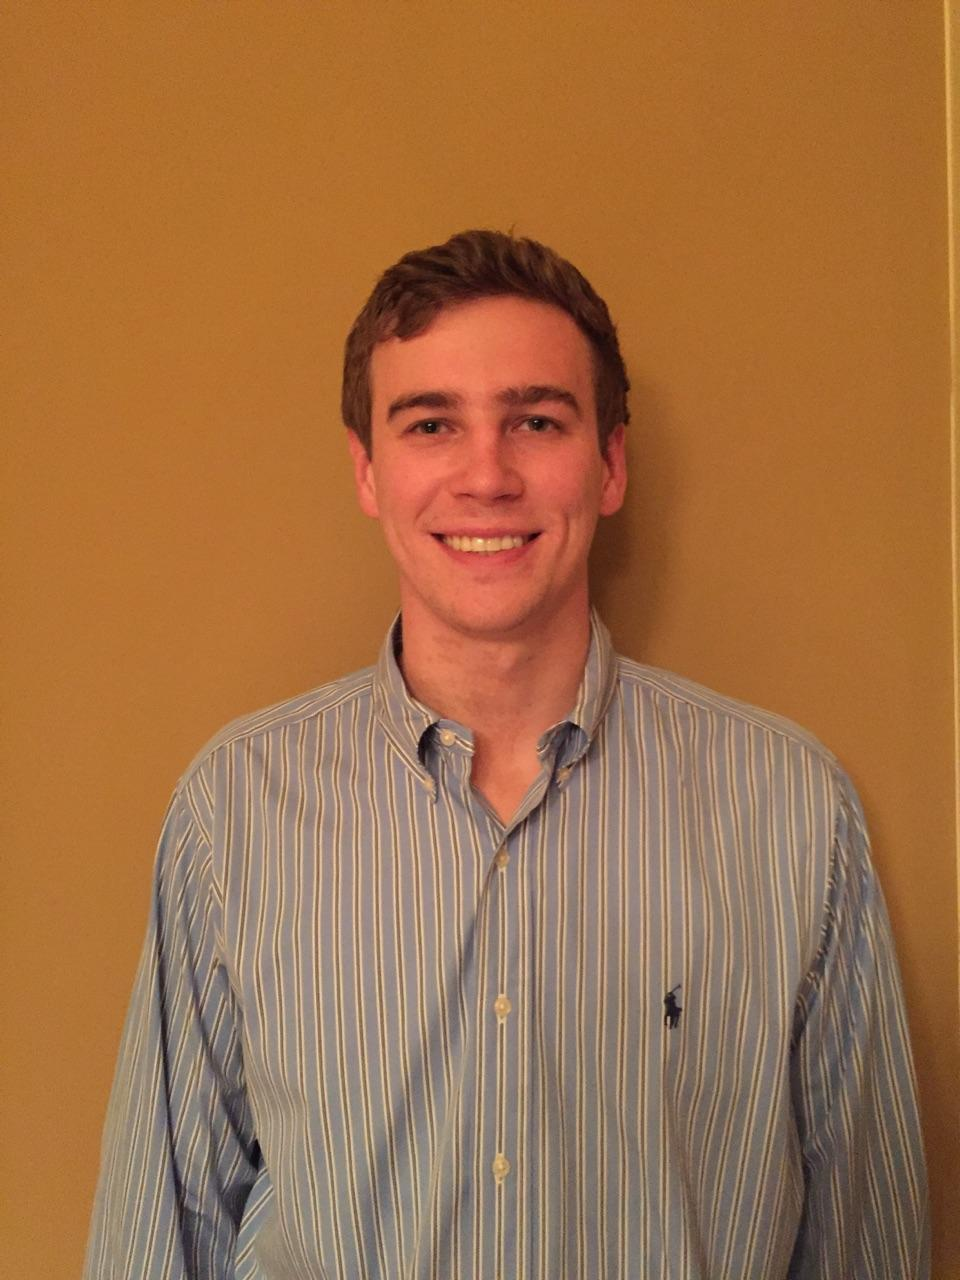
\includegraphics[width=1in,height=1.25in,clip,keepaspectratio]{jackson_parker}}{Jackson Parker}
\newline
M.S. Student with an Emphasis in Electrical and Computer Engineering, currently is the Systems Lead for the UGA Small Satellite Research Laboratory.
\end{IEEEbiography}%

% \vspace{10cm}

\begin{IEEEbiography}{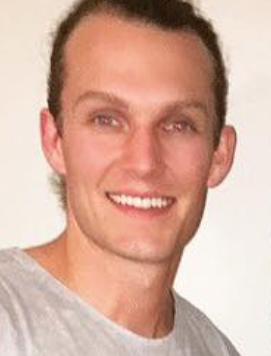
\includegraphics[width=1in,height=1.25in,clip,keepaspectratio]{allen_spain}}{Allen Spain}
\newline
\vspace{10cm}
\newline
M.S. Student with an Emphasis in Electrical and Computer Engineering, currently is the Lead Hardware Engineer for the Small Satellite Research Laboratory.
\end{IEEEbiography}

% \vspace{10cm}

\begin{IEEEbiography}{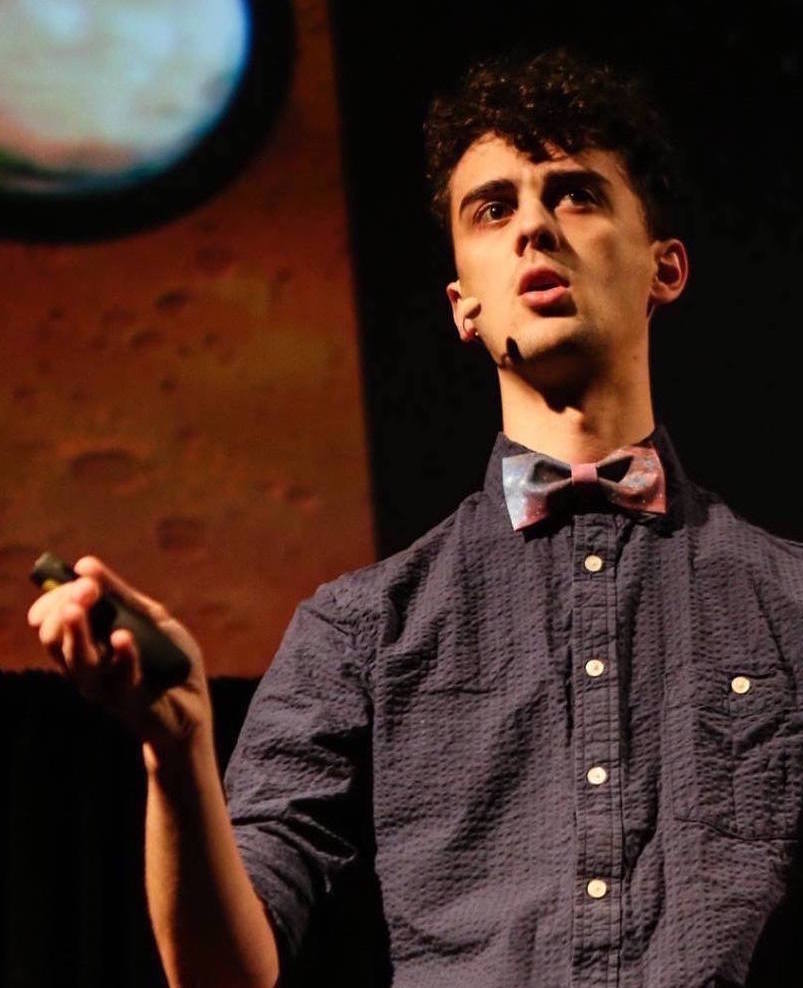
\includegraphics[width=1in,height=1.25in,clip,keepaspectratio]{caleb_adams}}{Caleb Adams}
\newline
Ph.D. Student in the department of Computer Science, is the Co-Founder of the Small Satellite Research Laboratory.
\end{IEEEbiography}

%end of doc


\end{document}
